% file: 2-11-heapsort/heapsort-selection-worst-7.tex
% 7: containing 7 nodes
% This example is given in the answer to Ex.23 of Section 5.2.3 of TAOCP vol 3.

\documentclass[tikz]{standalone}
\usepackage{tikz-qtree}

\begin{document}
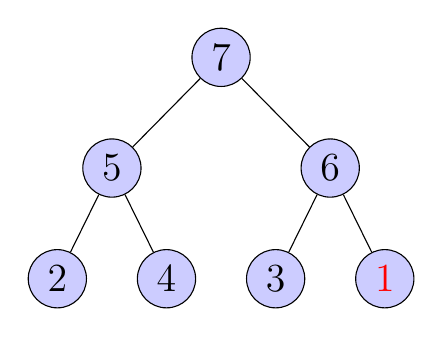
\begin{tikzpicture} [level distance = 40pt, sibling distance = 18pt,
  edge from parent/.style= { % added code
      draw, edge from parent path = {(\tikzparentnode) -- (\tikzchildnode)}}]
  \tikzset{every tree node/.style = 
    {align = center, circle, draw, fill = blue!20, font = \Large}}
    \Tree [.$7$
	    [.$5$
	       $2$ 
	       $4$
            ]
	    [.$6$ 
	      $3$
	      \textcolor{red}{$1$}
	   ] 
        ]
\end{tikzpicture}
\end{document}
